\subsection{Prime-Time Ratio} \label{subsec:primetime}

ISPs design networks to handle peak demand, which is usually observed
during prime-time hours, when subscribers heavily consume real-time
entertainment traffic, such as video.  The FCC defines prime-time as the
local time from 7:00--11:00 p.m.~\cite{fcc2014measuring-broadband}. To
measure the concentration of network usage during prime-time, we use
Sandvine's definition of the \emph{prime-time ratio}: the ratio of the
average (hourly) traffic demand during prime-time hours to the average
demand in non-prime-time hours~\cite{sandvine20141h, sandvine20142h}.
We measured the prime-time ratio of the subscribers in the control and
treatment groups considering each contiguous four-hour period in each
day. Our experiment shows that, in fact, the evening hours with the
largest prime-time ratio are 8:00~p.m.--12:00~a.m., so we use this time
interval for our definition of prime time.

%\begin{figure}[t]
%\begin{minipage}{1\linewidth}
%\centering
%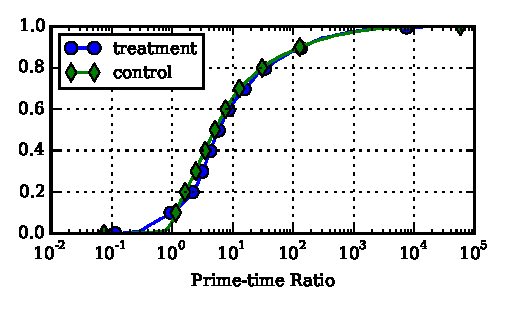
\includegraphics[width=1\linewidth]{figures/prime-time-ratio-per-device-cdf-MEAN.pdf}
%\caption{Prime-Time Ratio\label{fig:cdf-prime-time-ratio}}
%\end{minipage}
%\end{figure}

%\begin{subfigure}[]{.32\linewidth}
%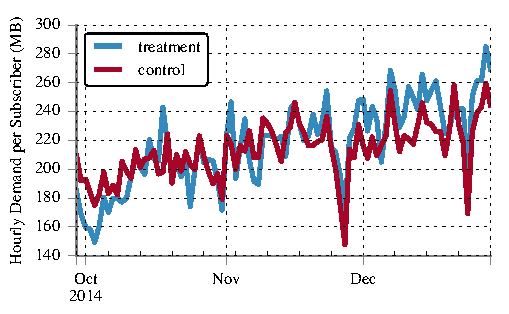
\includegraphics[width=1\linewidth]{figures/primetime_usage_per_day_per_subs.pdf}
%\caption{\label{fig:pt}}
%\end{subfigure}

%\begin{subfigure}[b]{.32\linewidth}
%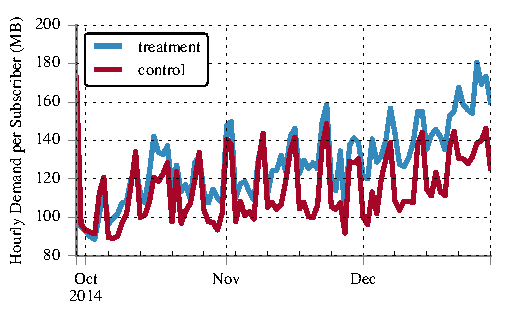
\includegraphics[width=1\linewidth]{figures/nonprimetime_usage_per_day_per_subs.pdf}
%\caption{\label{fig:non-pt}}
%\end{subfigure}

\begin{table}[t]
\centering
\begin{tabular}{| cc | c |c | }\hline
  &                    & Weekday         & Weekends \\\hline
\multirow{2}{*}{\begin{tabular}[c]{@{}l@{}}Hourly Traffic in\\ Prime-Time\end{tabular}}
& treatment          & 233.12          & 246.93   \\
& control            & 225.40          & 238.15   \\\hline
\multirow{2}{*}{\begin{tabular}[c]{@{}l@{}}Hourly Traffic in\\ Non-Prime-Time\end{tabular}}
& treatment & 124.18 & 143.08    \\
& control   & 104.30  & 133.16  \\\hline
\multirow{2}{*}{\begin{tabular}[c]{@{}l@{}}Prime-Time Ratio\end{tabular}}
& treatment & {1.88} &  1.73 \\
& control  &  {2.16} &  1.79 \\\hline
\end{tabular}
\caption{Hourly traffic demand during  prime-time hours (MB).\label{tab:prime-time-demand}}
\end{table}


Table~\ref{tab:data-stats} shows that the average hourly prime-time downstream traffic per
1,000 subscribers is
209.5 GB for the treatment group, compared to 205.1 GB for the control
group, about a 2\% increase. 
\f{In contrast, during an average hour
{\em outside} of prime time, the traffic per 1,000 subscribers is 122.3
GB for the treatment group, compared to
108.5 GB for the control group, amounting to about a 12\% increase.} This
more significant difference in demand during hours outside of the
daily prime-time is also apparent from the weekly usage patterns in
Figure~\ref{fig:traffic-demand-timeseries}. 

We also calculated the prime-time ratio per day over weekends and
weekdays, as shown in Table \ref{tab:prime-time-demand}.  On weekends,
the prime-time ratios for the treatment and control groups are 1.73 and
1.79 respectively. On the weekdays, the prime-time ratio for the control
group is 2.16 compared to 1.88 for the treatment group. 
\f{In terms of
absolute demand, the prime-time demand
on weekdays in the treatment group is within 4\%
of that in the control group. In contrast, the demand in
{\em non-prime-time hours} is 19\% higher for the treatment group on weekdays,
and only 7.5\% higher on weekends.} The increased non-prime-time demand in the
control group suggests that many of the users in both the control and
treatment groups (\ie, those subscribers who are already on high service
tiers) may in fact be subscribers who work from home and thus increase
their demand more during non-prime-time and weekdays as a result of the
service tier upgrade..

While 6\% of the subscribers in both groups had a prime-time ratio over
100, we also observed that 9\% of the control group and 14\% of the
treatment group had prime-time ratios {\em less than 1}, indicating that
these users actually had higher demand during the day than they did
during prime time. Similarly, these users may be small home
businesses or subscribers who work at home.


\if 0
For our dataset, the prime-time ratio for the treatment and control groups
were 1.70 and 1.93 respectively. By definition, the prime-time ratio is measured using
total traffic volume in a day. However, not all subscribers contribute equally
to the traffic volume. We observed that the median \emph{prime-time ratio per subscriber}
is 3.39 for the \treatment{} group and 2.91 for the \control{} group. 
The prime time ratio of the higher tier is more than the lower tier when calculated per
subscriber, but by volume it is the inverse.
The overall demand of subscribers in \treatment{} has increased substantially
on a per-subscriber basis, although the total volume does not show the same increase.
This result indicates that individual subscribers that do not contribute substantially
to the traffic volume are the ones who have higher usage in prime-time as compared to their
lower tier counterparts.
\fi

